\documentclass[]{article}
\usepackage{hyperref}
\usepackage{graphicx}
\hypersetup{
	colorlinks=true,
	linkcolor=blue,
	filecolor=magenta,      
	urlcolor=cyan,
	pdftitle={Overleaf Example},
	pdfpagemode=FullScreen,
}
\newcommand{\quotes}[1]{``#1''}
%opening
\title{Movies Visual Analysis}
\author{Luca Giovannesi}

\begin{document}

\maketitle

\section{Introduction}
IMDB is a website in which all moves data are collected, but, there isn't a built-in visual tool to analyzed these data, to analyze the data we have to open multiple pages and comparing data in a manual way.\newline
The main use cases for this software could be:
\begin{itemize}
	\item To discover new movies based by some criteria
	\item To discover new movies or similar to movies that you had already seen and you had like.
	\item To find trends, insights and curiosities on a large dataset of movies
 
	
\end{itemize}
\section{Related work}
\section{Dataset}
\subsection{The used dataset}
The used dataset is the one called \quotes{\href{https://www.kaggle.com/datasets/rounakbanik/the-movies-dataset}{The Movies Dataset}} available on Kaggle, this dataset contains about 5000 movies from the 1917 until 2017.\newline
The dataset is composed by 7 csv files, but we use only 3 of them:
\begin{itemize}
	\item \textbf{\quotes{movie\_metadata.csv}}: This file has 24 columns and it contains the main information of the movies.
	\item \textbf{\quotes{keywords.csv}}: This file includes the keywords of each movies.
	\item \textbf{\quotes{credits.csv}}: This file contains information about the people who worked on the movies. 
\end{itemize}
\subsection{Dataset processing}
The dataset needs a data elaboration to create a new dataset customized for our tool, in this way we avoid to perform heavy computation in \quotes{realtime} in the visualization tool and we drop the useless data in order to have a small dataset with a quicker loading time.\newline
This pre-processing phase is made by a python script and it is composed by 2 main phases:
\begin{enumerate}
	\item In this phase we merge all the data from the different files and we drop the movies which contains invalid data, like empty fields or invalid formats.
	\item This step computes the needed information for the multidimensional reduction, it is subdivided in 2 sub-phases:
	\begin{enumerate}
		\item \textbf{Build of similarity matrix}\newline
		 We have build a similarity matrix in which each cell $ij$ is filled with the similarity between the keywords of the movies $i$ and $j$
		\item \textbf{MultiDimensional Scaling positions}\newline
		Starting from the similarity matrix we compute the position of each movie in the multidimensional scaling plot.
	\end{enumerate}
\end{enumerate}
After the previous elaboration we have for each movie these fields:
\begin{itemize}
	\item \textbf{id} An integer used to identify the movies.
	\item \textbf{Title} The original title of the movies.
	\item \textbf{Genres} The genres of the movies.
	\item \textbf{Release year} The release year of the movies.
	\item \textbf{Runtime} The runtime in minutes.
	\item \textbf{Spoken languages} The spoken languages of the movies.
	\item \textbf{Vote avg} The average of the votes.
	\item \textbf{Vote count} The amount of the votes.
	\item \textbf{Revenue} The revenue in dollars.
	\item \textbf{Popularity} A popularity decimal value assigned by IMDB.
	\item \textbf{Budget} The budget in dollars.
	\item \textbf{Keywords}	The keywords of each movies, they are not directly used by the tool, but they can be useful to understand if the MDS works well.
	\item \textbf{MDS position} The coordinates of each movie in the MDS plot.
	\item \textbf{Director} The movie's director.
\end{itemize}
So we have 14 fields and 4943 movies, this makes the AS index equal to $69202$ definitely bigger than the suggested one, so we have created also the option to filter the dataset taking only the top 1000 movies by popularity, with this smaller dataset we have an AS index of $1400$ giving a smoother user interaction, expacially on low-end PC.\newline
\section{Visualization Techniques}
\subsection{Main interface}
The tool include a short header with the project name and an option to select the two type of dataset, can be selected the full dataset with about 5000 movies or the smaller one with only the top 1000 movies by popularity.\newline
Since the dataset has a dimension of about 5 MB, the loading of the page can take some time if the user has a slow internet connection, so there is also a nice interface shown in the loading phase.
\subsection{Multidimensional scaling}
\begin{figure}[h!]
	\centering
	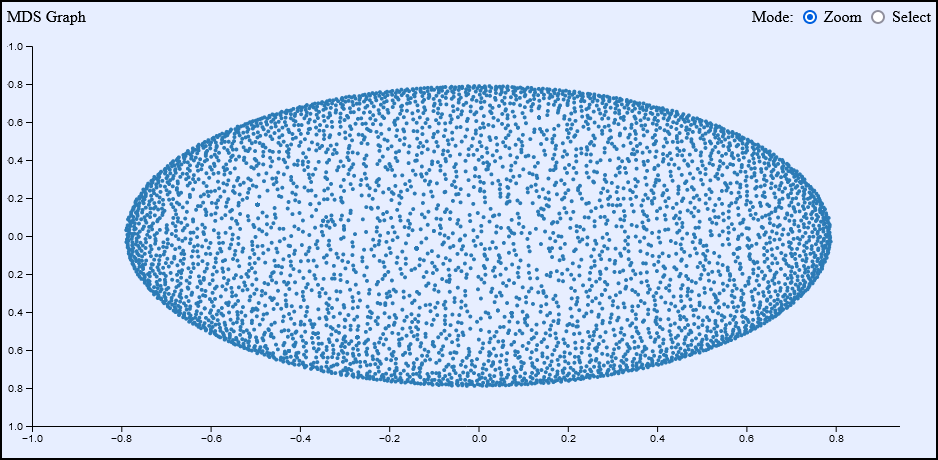
\includegraphics[width=1\linewidth]{images/mds_plot}
	\caption{Multidimensional plot}
	\label{fig:mdsplot}
\end{figure}
\subsubsection{Pre-Processing phase}
Multi-dimension scaling is a technique to show graphically the similarity between a set of elements, starting from a similarity matrix in which we have an item for each row and column, we can use an appropriate algorithm to set a position of the element in a N-dimensions space, in our case into a 2D space.\newline
In this project we compute the similarity using the Jaccard distance between the keywords of each movies, the Jaccard distance is defined as $J(A,B)=\frac{|A\cap B|}{|A\cup B|}$, initially we have tried to use the cosine similarity but we had bad results, while with the Jaccard distance the outcomes are definitely better.\newline
Each movie has a set of keywords, each keyword has also an associated id, so for each movies is easy to get a vector with all the associated ids of the keywords, avoiding addition processes to have the keywords as numbers, from these vector of integers we can apply the Jaccard distance to get the similarity between the set of keywords.\newline
Once we have the similarity matrix we have used the sklearn.MDS function with parameters max\_iter=1000, dissimilarity="precomputed", n\_init=8, eps=1e-6, to computes the position in the 2D plane for each movie.\newline
The described computations are not done in real time by the webpage, because they are processes which took a lot of time, so they are done previusly with a python script in order to have inside the dataset directly the outcome helpful to draw this graph.
\subsubsection{Visualization tool}
In graph we have a set of dots, each dots represents a movie, the user can hover the mouse on a dot to see addition information (Movie title, Director and release year) and to highlight the movie on the other plots.\newline
The visualization tool has two modes: the zoom mode and the select mode, with the zoom mode the user can zoom and move the visualized area of the graph, while in select mode the user can select an area drawing a rectangle.


\subsection{Parallel coordinates}
\subsection{Bubble plot}
\subsection{Column plot}
\subsection{Selection list}
\subsection{Interaction}
\section{Insights}
\section{Conclusion}
\end{document}
